%!TEX root = mainfile.tex

\section{Lower Redshift limit on Re-ionization} % (fold)
\label{sec:lower_redshift_limit_on_Re-ionization}
	In the project the way that the lower redshift limit has been calculated is to first calculate the rate of photons capable of ionizing a hydrogen atom via equation~(\ref{eq:rate_of_ionising_photons})\cite{2010Natur.468...49R}.
	\begin{align}
		\frac{\d{n_{ion}}}{\d{t}}=f_{esc}\zeta\rho_\text{SFR}\label{eq:rate_of_ionising_photons}
	\end{align}
	Where $f_{esc}$ is the fraction of ionizing photons that escape a galaxy, $\zeta$ is the number of hydrogen-ionizing photons produced per second per unit star formation rate, see Section~\ref{sub:reionization_parameters}, and $\rho_\text{SFR}$ is the star formation rate per unit volume.

	Therefore by integrating this equation up to the age of the universe at a specific redshift a total number of photons capable of ionizing the universe can be outputted. The number of ionizing photons are then equated to the total number of hydrogen atoms in the IGM of the universe to obtain a lower redshift limit of reionization.

	First of all the program calculates the critical density of the universe by,
	\begin{align}
		\rho_{crit}(z)=\frac{3H{(z)}^{2}}{8\pi G}
	\end{align}
	Then by multiplying this by the baryonic density parameter, $\Omega_{b}=0.045\pm0.004$, the baryonic density is achieved. Then, by multiplying by the fraction of hydrogen, calculated from big bang nucleosynthesis, the total density of hydrogen in the universe can be obtained.

	From the 7 year WMAP survey\cite{2011ApJS..192...18K}, the primordial Helium fraction was found to be $Y=0.33\pm0.09$. Where it is assumed that Hydrogen fraction ($X$) is simply $1-Y$ (therefore 0 metallicity). Nevertheless as a simplifying assumption it is not too bad as the errors on fraction of helium are higher than the actual fraction of heavier elements.

	Then finally dividing the mass density of hydrogen by the atomic mass unit the code obtains a number density of hydrogen. In the code a redshift time relation $\frac{1}{(1+z)}\propto t^{2/3}$, assuming a matter dominated universe, is used and therefore,
	\begin{align}
		t &= \frac{t_{0}}{{(1+z)}^{3/2}} \\
		\Rightarrow \dx{t}{z} &= \frac{3}{2}\frac{t_{0}}{{(1+z)}^{5/2}}
	\end{align}

	In the first version of the code, values of star formation rate densities from  various articles with redshifts varying from redshifts 4 to up to about 8 from\cite{2010MNRAS.401.2561W}, which determine star formation rates from observations of Gamma-ray bursts (GRBs) from deaths of massive short lived stars which can be directly related to star formation rate. Also compiling these values with those from\cite{2012ApJ...759L..38A}, which use a semi-analytical model to determine star formation rates from redshifts 9 to 16. These two papers with very different methods have surprising correlation in values.

	These values were then plotted against redshift. The function of redshift that was used for $\rho_\text{SFR}$ was
	\begin{align}
		\rho_\text{SFR}(z)=0.399(\pm 0.181)\e{-0.253(\pm 0.118)z}-0.011(\pm 0.025)
	\end{align}
	However this equation only works up to a redshift of around 5 as the star formation rate for galaxies drops with redshifts lower than this due to the gas being used up and star formation dropping off. This should not effect the results too much however as the project tends to study redshifts higher than this anyway. Also there are be large errors on higher redshift values due to problems with extrapolating the data, and unrealistic numbers of star formation where in reality there would be none. The values of $f_\text{esc}=0.2$ and $\zeta=10^{53.5}$ as stated in sections~\ref{sub:escape_fraction} and~\ref{sub:hydrogen_ionizing_photons_produced_per_second_per_unit_star_formation_rate} were applied here.

	The code also used a function of the global stellar mass density to figure out the amount of hydrogen that was calculated was in stars at a given redshift. This therefore gives a certain fraction that is not part of the IGM and does not need to be ionized. These values were taken from the direct observations of three papers \cite{2006AA...459..745F}, \cite{2003A&A...401...73W} and \cite{2003ApJS..149..289B}. The function of redshift that was calculated was
	\begin{align}
		\rho_\text{stellar}(M_{\odot}\si{\per\mega\parsec\cubed})=\e{-0.81z+19.7}
	\end{align}
	but this does not have much effect on the number of hydrogen as the stellar fraction is very small, so this is not a significant contributing factor.

	The code then loops for different values of redshift from redshift 25 at redshift intervals of 0.1, calculating the number of ionizing photons at those different epochs and equating this to the hydrogen number. This then outputs ionized fraction against redshift, shown in Figure~\ref{fig:IonizedFraction1}.
	\begin{figure}[htbp]
		\centering
			\begingroup\endlinechar=-1
		  		\resizebox{0.7\textwidth}{!}{%
					% GNUPLOT: LaTeX picture with Postscript
\begingroup
  \makeatletter
  \providecommand\color[2][]{%
    \GenericError{(gnuplot) \space\space\space\@spaces}{%
      Package color not loaded in conjunction with
      terminal option `colourtext'%
    }{See the gnuplot documentation for explanation.%
    }{Either use 'blacktext' in gnuplot or load the package
      color.sty in LaTeX.}%
    \renewcommand\color[2][]{}%
  }%
  \providecommand\includegraphics[2][]{%
    \GenericError{(gnuplot) \space\space\space\@spaces}{%
      Package graphicx or graphics not loaded%
    }{See the gnuplot documentation for explanation.%
    }{The gnuplot epslatex terminal needs graphicx.sty or graphics.sty.}%
    \renewcommand\includegraphics[2][]{}%
  }%
  \providecommand\rotatebox[2]{#2}%
  \@ifundefined{ifGPcolor}{%
    \newif\ifGPcolor
    \GPcolortrue
  }{}%
  \@ifundefined{ifGPblacktext}{%
    \newif\ifGPblacktext
    \GPblacktexttrue
  }{}%
  % define a \g@addto@macro without @ in the name:
  \let\gplgaddtomacro\g@addto@macro
  % define empty templates for all commands taking text:
  \gdef\gplbacktext{}%
  \gdef\gplfronttext{}%
  \makeatother
  \ifGPblacktext
    % no textcolor at all
    \def\colorrgb#1{}%
    \def\colorgray#1{}%
  \else
    % gray or color?
    \ifGPcolor
      \def\colorrgb#1{\color[rgb]{#1}}%
      \def\colorgray#1{\color[gray]{#1}}%
      \expandafter\def\csname LTw\endcsname{\color{white}}%
      \expandafter\def\csname LTb\endcsname{\color{black}}%
      \expandafter\def\csname LTa\endcsname{\color{black}}%
      \expandafter\def\csname LT0\endcsname{\color[rgb]{1,0,0}}%
      \expandafter\def\csname LT1\endcsname{\color[rgb]{0,1,0}}%
      \expandafter\def\csname LT2\endcsname{\color[rgb]{0,0,1}}%
      \expandafter\def\csname LT3\endcsname{\color[rgb]{1,0,1}}%
      \expandafter\def\csname LT4\endcsname{\color[rgb]{0,1,1}}%
      \expandafter\def\csname LT5\endcsname{\color[rgb]{1,1,0}}%
      \expandafter\def\csname LT6\endcsname{\color[rgb]{0,0,0}}%
      \expandafter\def\csname LT7\endcsname{\color[rgb]{1,0.3,0}}%
      \expandafter\def\csname LT8\endcsname{\color[rgb]{0.5,0.5,0.5}}%
    \else
      % gray
      \def\colorrgb#1{\color{black}}%
      \def\colorgray#1{\color[gray]{#1}}%
      \expandafter\def\csname LTw\endcsname{\color{white}}%
      \expandafter\def\csname LTb\endcsname{\color{black}}%
      \expandafter\def\csname LTa\endcsname{\color{black}}%
      \expandafter\def\csname LT0\endcsname{\color{black}}%
      \expandafter\def\csname LT1\endcsname{\color{black}}%
      \expandafter\def\csname LT2\endcsname{\color{black}}%
      \expandafter\def\csname LT3\endcsname{\color{black}}%
      \expandafter\def\csname LT4\endcsname{\color{black}}%
      \expandafter\def\csname LT5\endcsname{\color{black}}%
      \expandafter\def\csname LT6\endcsname{\color{black}}%
      \expandafter\def\csname LT7\endcsname{\color{black}}%
      \expandafter\def\csname LT8\endcsname{\color{black}}%
    \fi
  \fi
  \setlength{\unitlength}{0.0500bp}%
  \begin{picture}(7200.00,4320.00)%
    \gplgaddtomacro\gplbacktext{%
      \put(747,595){\makebox(0,0)[r]{\strut{} 0}}%
      \put(747,1182){\makebox(0,0)[r]{\strut{} 0.2}}%
      \put(747,1768){\makebox(0,0)[r]{\strut{} 0.4}}%
      \put(747,2355){\makebox(0,0)[r]{\strut{} 0.6}}%
      \put(747,2942){\makebox(0,0)[r]{\strut{} 0.8}}%
      \put(747,3528){\makebox(0,0)[r]{\strut{} 1}}%
      \put(747,4115){\makebox(0,0)[r]{\strut{} 1.2}}%
      \put(849,409){\makebox(0,0){\strut{} 0}}%
      \put(2058,409){\makebox(0,0){\strut{} 5}}%
      \put(3267,409){\makebox(0,0){\strut{} 10}}%
      \put(4475,409){\makebox(0,0){\strut{} 15}}%
      \put(5684,409){\makebox(0,0){\strut{} 20}}%
      \put(6893,409){\makebox(0,0){\strut{} 25}}%
      \csname LTb\endcsname%
      \put(144,2355){\rotatebox{-270}{\makebox(0,0){\strut{}Ionised Fraction ($X$)}}}%
      \csname LTb\endcsname%
      \put(3871,130){\makebox(0,0){\strut{}Redshift (z)}}%
      \put(3871,4022){\makebox(0,0){\strut{}}}%
    }%
    \gplgaddtomacro\gplfronttext{%
      \csname LTb\endcsname%
      \put(6105,3948){\makebox(0,0)[r]{\strut{}Best Fit}}%
      \csname LTb\endcsname%
      \put(6105,3762){\makebox(0,0)[r]{\strut{}Lower Limit}}%
      \csname LTb\endcsname%
      \put(6105,3576){\makebox(0,0)[r]{\strut{}Upper Limit}}%
    }%
    \gplbacktext
    \put(0,0){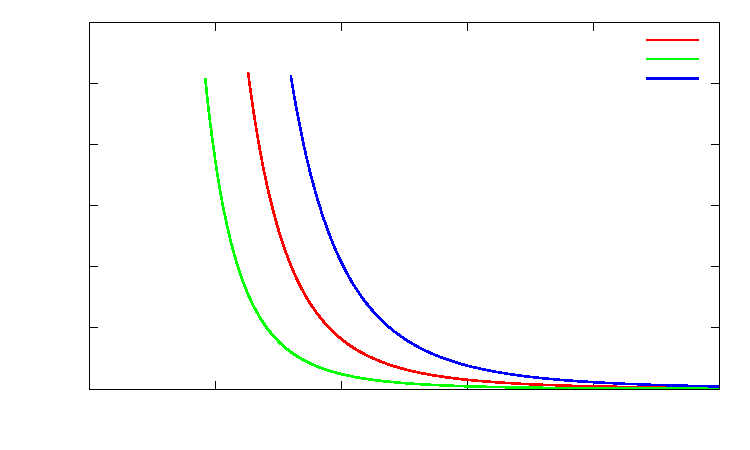
\includegraphics{GRAPH_StellarDens_exponential}}%
    \gplfronttext
  \end{picture}%
\endgroup

		  		}\endgroup
		\caption{Plot of modeled ionized fraction of the IGM as a function of redshift.\label{fig:IonizedFraction1}}
	\end{figure}

	This implies that the universe is completely ionized at a redshift $6.3\pm1.7$, ignoring the rather large errors, this number is not a bad estimate of the epoch. This is known from articles which show from observations of Lyman-$\alpha$ emitters that there must be a large ionized fraction at $z=6.5$, due to attenuation from neutral hydrogen\cite{Ota:arXiv0707.1561}. Various theoretical models of star formation rate predict a ionized universe at around $z=6$ and it is stated that the Sunyaev-Zeldovich effect has limited the end of reionization to earlier than $z=5.8$\cite{2012MNRAS.423..862K}. Therefore we have a predicted epoch of reionization of $5.8<z<6.5$ from the literature.

	However as recombination has not been included which will slow down the rate at which the universe is ionized, as it is effectively the opposite effect of reionization. Or the fact that both the escape fraction and $\zeta$ are likely to change with redshift, makes this number is not entirely realistic.

	\subsection{Reionization Parameters} % (fold)
	\label{sub:reionization_parameters}
		When calculating the rate of re-ionizing photons, there are two important constants to be considered. These are the escape fraction of photons emitted by young stars which manage to escape from the galaxy, $f_\text{esc}$, and the number of hydrogen ionizing photons produced per second per unit star formation rate, $\zeta$. Throughout this project, well established values have been used nevertheless it is still important to understand how these values are obtained.
	% subsection reionization_parameters (end)

		\subsubsection{Escape Fraction} % (fold)
		\label{sub:escape_fraction}
			This value is the escape fraction of photons. If this number were one then every single photon that's produced would escape from the galaxy into the IGM to contribute to the ionization of the neutral hydrogen however this is not the case. This figure is in fact much smaller meaning that most of the photons never reach the IGM at all. This is due to the neutral hydrogen within the galaxy itself absorbing the photons before they can escape. The amount of neutral hydrogen, the density and size of the galaxy and whether or not the galaxy is part of a cluster all contribute to the value of fesc and hence it is notoriously difficult to determine.

			It is often obtained by measuring the flux of UV photons below the Lyman limit of \SI{912}{\angstrom} which emerge from galaxies using methods such as intrepid spectroscopic and narrow-band imaging\cite{robertson2010early}. This is because only a certain fraction of the photons that were produced do emerge having managed to avoid interaction with the neutral gas within the galaxy thus measuring this flux directly and making assumptions of how many were initially produced would result in an estimate of the escape fraction. This comes with its own difficulties as often those photons which have managed to escape the galaxy are further absorbed by the IGM along the line of sight, reducing the flux that can be observed. This method relies on observations it has not been possible to determine the escape value for high redshift galaxies and so it has been extrapolated back to earlier cosmic times in Section~\ref{sub:evolving_escape_fraction}. As this value is so difficult to determine and varies from galaxy to galaxy it hasn't been confirmed but instead has been constrained so hence this project will trial a range of these values to see how this can affect the rate of re-ionizing photons. Robertson et al.'s 2010 paper estimates this value to lie within the range $0.1\lesssim f_\text{esc}\lesssim 0.2$\cite{robertson2010early} whereas Inoue (2006) claims that ``fesc increases from a value less than 0.01 at $z\le 1$ to about 0.1 at $z\ge 4$''\cite{inoue2006escape}. Furthermore there isn't enough data available to determine this to a great deal of accuracy and hence the extrapolated value for the escape fraction at high redshifts would be an approximation. As the value for the escape fraction can only vary from 0 to 1 its exact value cannot greatly alter the outcome of the calculation and thus an approximate value is sufficient within the realms of this project.

			The escape fraction can also be determined using galaxy formation simulations which is exactly what was done by Wood and Loeb in 2000. They found that the escape fraction at $z\approx 10$ is $\le1$\% for stars\cite{gnedin2008escape}. Calculating the escape fraction of ionizing photons from disk galaxies as a function of galaxy mass and redshift requires a complex code and that certain assumptions be made. These are that the gas in the disks is isothermal and radially exponential and that the source of radiation is either the stars within the disks or a central quasar. The mechanics of the program extend well beyond the scope of this project however the outcome of $f_\text{esc}=0.01$ is of use. As this particular paper was published in 2000 and has made relatively idealistic assumptions its legitimacy nowadays can be questioned. Therefore for the purposes of this project the observed values of $f_\text{esc}\approx 0.2$ were initially used with its evolution with redshift incorporated later.
		% subsection escape_fraction (end)

		\subsubsection{Hydrogen Ionizing Photons Produced ($s^{-1}M_\odot^{-1}\text{yr}$)} % (fold)
		\label{sub:hydrogen_ionizing_photons_produced_per_second_per_unit_star_formation_rate}
			The number of hydrogen ionizing photons produced per second per unit star formation rate is a very difficult number to pinpoint as it is not obvious how it could be determined numerically or observationally. This is because it is heavily dependent upon the characteristics of the star and, as each star is unique and stars themselves are so numerous, this becomes a very complex situation to simulate and thus it is common to take a representative average value for $\zeta$. Furthermore at the high redshifts considered in this project the stars are so far away that much bigger objects such as galaxies must instead be observed making it near-enough impossible to establish the activity of a single star.

			For the purposes of this project it has been assumed that $\zeta=10^{53.5}$\si{s^{-1}.M_{\odot}^{-1}.yr^{-1}}\cite{robertson2010early}. This particular value has been realised through the same detection methods as the escape fraction however as with fesc its precise value remains uncertain.

			The value for $\zeta$ can also be obtained numerically; more detail is included in Schull's 2011 paper\cite{shull2012critical}. This applies a very complicated method however it essentially converts the star formation rate density into numbers of OB sequence stars and computes the total number of ionizing photons produced by a star of a certain mass over its lifetime. Combining this with the rate at which stars of this mass are formed would give a good estimate for $\zeta$. As this method is highly complex it is not clear to what extent it relates to the specifics of this project and hence although it is a highly advanced way of calculating $\zeta$ it is perhaps more sensible for the value obtained in Robertson to be used as this is a very common and better understood figure.
		% subsection hydrogen_ionizing_photons_produced_per_second_per_unit_star_formation_rate (end)

	\subsection{Evolving Escape Fraction} % (fold)
	\label{sub:evolving_escape_fraction}
		As already stated the previous results make a basic assumption of of the escape fraction to be about $20\%$ during the epoch of reionization. This is obviously not a very good assumption as it will evolve with redshift. However there lies a problem in this which is related to the previous section, Section~\ref{sub:escape_fraction} which explained the difficulty in measuring this parameter as well as the problems in extrapolating out to higher redshifts much like in our star formation rates. This uncertainty in the measurement is what leads to the differences stated in\cite{2012ApJ...759L..38A}, which states a higher fraction at higher redshift due to lack of dust, and\cite{2000ApJ...545...86W} which states the opposite, due to increasing disk densities and increasing density in the universe as a whole. However from\cite{2012arXiv1209.2123F} and\cite{2013MNRAS.428L...1M} by using recent semi-analytical models they found that the escape fraction does indeed increase with redshift and so this is the model that is used in this project.

		Once again using the fit program to fit a exponential to the escape fraction measurements and predictions from\cite{2012ApJ...759L..38A},\cite{2006ApJ...651L..89R} and\cite{2006MNRAS.371L...1I}. The functional form that is achieved is
		\begin{align}
			f_\text{esc}(z)=\e{0.013\pm0.011-0.952\pm0.06}
		\end{align}
		The code is then run again with this escape fraction instead of the constant $20\%$, the results achieved are shown in \ref{fig:IonizedFraction2}
		\begin{figure}[htbp]
			\centering
				\begingroup\endlinechar=-1
					\resizebox{0.7\textwidth}{!}{%
						% GNUPLOT: LaTeX picture with Postscript
\begingroup
  \makeatletter
  \providecommand\color[2][]{%
    \GenericError{(gnuplot) \space\space\space\@spaces}{%
      Package color not loaded in conjunction with
      terminal option `colourtext'%
    }{See the gnuplot documentation for explanation.%
    }{Either use 'blacktext' in gnuplot or load the package
      color.sty in LaTeX.}%
    \renewcommand\color[2][]{}%
  }%
  \providecommand\includegraphics[2][]{%
    \GenericError{(gnuplot) \space\space\space\@spaces}{%
      Package graphicx or graphics not loaded%
    }{See the gnuplot documentation for explanation.%
    }{The gnuplot epslatex terminal needs graphicx.sty or graphics.sty.}%
    \renewcommand\includegraphics[2][]{}%
  }%
  \providecommand\rotatebox[2]{#2}%
  \@ifundefined{ifGPcolor}{%
    \newif\ifGPcolor
    \GPcolortrue
  }{}%
  \@ifundefined{ifGPblacktext}{%
    \newif\ifGPblacktext
    \GPblacktexttrue
  }{}%
  % define a \g@addto@macro without @ in the name:
  \let\gplgaddtomacro\g@addto@macro
  % define empty templates for all commands taking text:
  \gdef\gplbacktext{}%
  \gdef\gplfronttext{}%
  \makeatother
  \ifGPblacktext
    % no textcolor at all
    \def\colorrgb#1{}%
    \def\colorgray#1{}%
  \else
    % gray or color?
    \ifGPcolor
      \def\colorrgb#1{\color[rgb]{#1}}%
      \def\colorgray#1{\color[gray]{#1}}%
      \expandafter\def\csname LTw\endcsname{\color{white}}%
      \expandafter\def\csname LTb\endcsname{\color{black}}%
      \expandafter\def\csname LTa\endcsname{\color{black}}%
      \expandafter\def\csname LT0\endcsname{\color[rgb]{1,0,0}}%
      \expandafter\def\csname LT1\endcsname{\color[rgb]{0,1,0}}%
      \expandafter\def\csname LT2\endcsname{\color[rgb]{0,0,1}}%
      \expandafter\def\csname LT3\endcsname{\color[rgb]{1,0,1}}%
      \expandafter\def\csname LT4\endcsname{\color[rgb]{0,1,1}}%
      \expandafter\def\csname LT5\endcsname{\color[rgb]{1,1,0}}%
      \expandafter\def\csname LT6\endcsname{\color[rgb]{0,0,0}}%
      \expandafter\def\csname LT7\endcsname{\color[rgb]{1,0.3,0}}%
      \expandafter\def\csname LT8\endcsname{\color[rgb]{0.5,0.5,0.5}}%
    \else
      % gray
      \def\colorrgb#1{\color{black}}%
      \def\colorgray#1{\color[gray]{#1}}%
      \expandafter\def\csname LTw\endcsname{\color{white}}%
      \expandafter\def\csname LTb\endcsname{\color{black}}%
      \expandafter\def\csname LTa\endcsname{\color{black}}%
      \expandafter\def\csname LT0\endcsname{\color{black}}%
      \expandafter\def\csname LT1\endcsname{\color{black}}%
      \expandafter\def\csname LT2\endcsname{\color{black}}%
      \expandafter\def\csname LT3\endcsname{\color{black}}%
      \expandafter\def\csname LT4\endcsname{\color{black}}%
      \expandafter\def\csname LT5\endcsname{\color{black}}%
      \expandafter\def\csname LT6\endcsname{\color{black}}%
      \expandafter\def\csname LT7\endcsname{\color{black}}%
      \expandafter\def\csname LT8\endcsname{\color{black}}%
    \fi
  \fi
  \setlength{\unitlength}{0.0500bp}%
  \begin{picture}(7200.00,4320.00)%
    \gplgaddtomacro\gplbacktext{%
      \put(747,595){\makebox(0,0)[r]{\strut{} 0}}%
      \put(747,1235){\makebox(0,0)[r]{\strut{} 0.2}}%
      \put(747,1875){\makebox(0,0)[r]{\strut{} 0.4}}%
      \put(747,2515){\makebox(0,0)[r]{\strut{} 0.6}}%
      \put(747,3155){\makebox(0,0)[r]{\strut{} 0.8}}%
      \put(747,3795){\makebox(0,0)[r]{\strut{} 1}}%
      \put(849,409){\makebox(0,0){\strut{} 4}}%
      \put(1398,409){\makebox(0,0){\strut{} 6}}%
      \put(1948,409){\makebox(0,0){\strut{} 8}}%
      \put(2497,409){\makebox(0,0){\strut{} 10}}%
      \put(3047,409){\makebox(0,0){\strut{} 12}}%
      \put(3596,409){\makebox(0,0){\strut{} 14}}%
      \put(4146,409){\makebox(0,0){\strut{} 16}}%
      \put(4695,409){\makebox(0,0){\strut{} 18}}%
      \put(5245,409){\makebox(0,0){\strut{} 20}}%
      \put(5794,409){\makebox(0,0){\strut{} 22}}%
      \put(6344,409){\makebox(0,0){\strut{} 24}}%
      \put(6893,409){\makebox(0,0){\strut{} 26}}%
      \csname LTb\endcsname%
      \put(144,2355){\rotatebox{-270}{\makebox(0,0){\strut{}Ionised Fraction}}}%
      \csname LTb\endcsname%
      \put(3871,130){\makebox(0,0){\strut{}Redshift ($z$)}}%
      \put(3871,4022){\makebox(0,0){\strut{}}}%
    }%
    \gplgaddtomacro\gplfronttext{%
      \csname LTb\endcsname%
      \put(5658,3702){\makebox(0,0)[r]{\strut{}Ionised Fraction}}%
      \csname LTb\endcsname%
      \put(5658,3516){\makebox(0,0)[r]{\strut{}Upper Limit}}%
      \csname LTb\endcsname%
      \put(5658,3330){\makebox(0,0)[r]{\strut{}Lower Limit}}%
    }%
    \gplbacktext
    \put(0,0){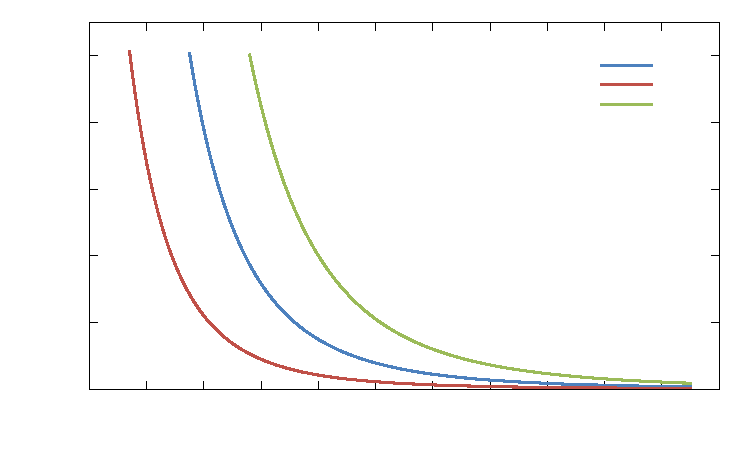
\includegraphics{GRAPH_SFR_ionised_fraction}}%
    \gplfronttext
  \end{picture}%
\endgroup

					}\endgroup
			\caption{Plot of modeled ionized fraction of the IGM as a function of redshift with predicting evolving escape fraction.\label{fig:IonizedFraction2}}
		\end{figure}

		The graph in Figure~\ref{fig:IonizedFraction2} shows that the addition of the evolving escape fraction has resulted in the universe being ionized quicker which is what is expected, since recombinations have not been included in this model. This model outputs a redshift of $7.5\pm2.1$, which shows the increase in redshift and also in error due to the error on $f_\text{esc}$ itself. It is very hard to determine whether this is an improvement or a hindrance to the previous model just due to the uncertainty on measuring/predicting $f_\text{esc}$, therefore it is hard to be certain of accuracy of the evolving form of $f_\text{esc}$.
	% subsection evolving_escape_fraction (end)

	% \subsection{Recombinations} % (fold)
	% \label{sub:recombinations}
	% %Not completed having trouble with it not sure if it should be included without conclusive results?
	% 	To include Recombinations into our project, the rate at which hydrogen will recombine. The recombination rate was found to be,
	% 	\begin{align}
	% 		\frac{dn_{rec}}{dt}=\frac{Q_{HII}}{\overline{t}_{rec}}
	% 	\end{align}
	% 	Where $\overline{t}_\text{rec}$ is the mean recombination time and $Q_\text{HII}$ is the ``volume filling factor''\cite{2012ApJ...746..125H}. The mean recombination time has the form,
	% 	\begin{align}
	% 		\overline{t}_{rec}= {\left(1.08\langle n_{H}\rangle\alpha_{B}C\right)}^{-1}
	% 	\end{align}
	% 	Where $C$ is the clumping factor the IGM, $\alpha_{B}$ is the recombination coefficent for excited states of hydrogen and the 1.08 accounts for the presence of photoelectrons from singly ionized helium. Where values of the clumping factor against redshift are cited from a theoretical model in\cite{2011MNRAS.412L..16R}.

	% 	The code then takes this equation for the mean recombination time of hydrogen and integrates the inverse of this from 0 to the specific $t(z)$. This will give us a mean total of hydrogen that will have recombined in that time period. However when this method is implemented into the code and ran, it outputs values of recombination that are insignificant because they are so low. This seems unphysical as we would expect the recombinations in the universe to be much higher than this and make a significant contribution to the rate at which the universe ionizes.
	% % subsection recombinations (end)

% section lower_redshift_limit_on_reionization (end)
